% !TEX root = ../Rom-abcd.tex
%% -----------------------------------------------------
%% -- Musterdatei für die Erstellung des Beitrags
%% -- zum Romseminar. Um ein einheitliches Aussehen zu ermöglichen:
%% -- Bitte die Definitionen nicht ändern. 
%% -- Stand: 2024/11/02
%% -----------------------------------------------------

%% -- Definitionen, damit die Eingabe einfacher wird
%% -- Bitte \renewcommand belassen und die entsprechenden Angaben
%% -- eintragen.
%% --
\renewcommand{\LongTitel}{Langform des Titels}
\renewcommand{\ShortTitel}{Kurzform des Titel}
\renewcommand{\AutorenBeitrag}{Autor1, Autor2 \& Autor3}

%% -- Kapitelüberschrift und Eintrag in TOC
%% -- Bitte hier nichts ändern
%% --
\addchap[\ShortTitel]{\LongTitel}
\addtocontents{toc}{\textsc{\AutorenBeitrag}}
\addtocontents{toc}{}

%% -- Kopfzeile 
%% -- Gerade Seiten : Autoren
%% -- Ungerade Seiten: Kurztitel
%% -- Bitte hier nichts ändern
%% --
\markleft{\textsc{\AutorenBeitrag}}	
\markright{\textsc{\ShortTitel}}	

%% -- Titelseite des Beitrags 
%% -- Bild: Bitte hier eins vom Vortrag nutzen --> autor-abcd.jpg
%% -- Namen der Vortragenden --> Autor1 etc. entsprechend anpassen
%% --
\begin{center}
	\textsc{\Large \AutorenBeitrag}\\[1.5em]
	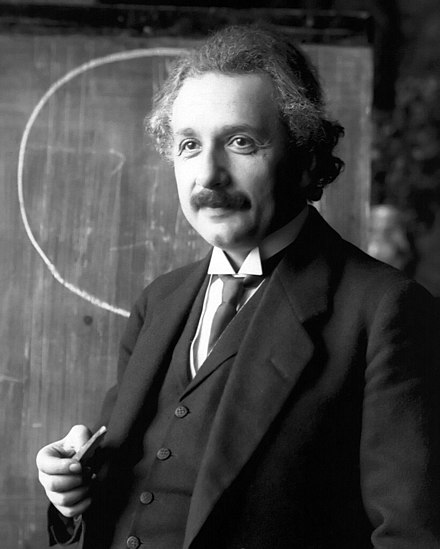
\includegraphics[width=8cm, height=8cm, keepaspectratio=true]{./content-abcd/autor-abcd.jpg}
\end{center}

%% -- Wer einen sinnvollen Spruch nutzen will
%% -- dann bitte mit \dictum[]{}; 
%% -- Anpassen der Breite: 
\renewcommand{\dictumwidth}{0.45\textwidth}
%% --

\dictum[\href{https://de.wikipedia.org/wiki/Albert_Einstein}{Albert Einstein}]{Wahnsinn ist, dasselbe immer  \mbox{wieder} zu tun und andere Ergebnisse zu erwarten.}

%%
\begin{quote}
Für eine kurze Zusammenfassung des Beitrags, damit man diesen unbedingt lesen will.
Aber lesen \emph{muss jeder} das README!!
\end{quote}

%% -- Literaturreferenzen des Beitrags am Ende des Artikels
%% -- Damit es keine Überscheidungen mit anderen Zitaten gibt
%% -- \begin{refsection} -- \end{refsection}
%% --
\begin{refsection}
%% --
\section*{Erster Hauptabschnitt}		%% 
\subsection*{Erster Unterabschnitt}		%% 

Eingabe von Text beginnt hier.
Jeden neuen Satz auf einer neuen Zeile beginnen -- macht das Lesen und die Fehlersuche einfacher.

Und einen neuen Absatz beginnt man, indem man eine Leerzeile einfügt. 
Bitte nicht \verb|\newline| oder \verb|\\| oder ähnliches dazu verwenden -- dies ist eine Todsünde in \LaTeX{}.

Literatur zitiert man mithilfe von \verb|\texcite[genaue Stelle]{label}| am Ende eines Satzes, \zB \ldots Interssant sind \textcite{AlphaGo}, \textcite{alsina:2013},  \textcite[S.\,120]{heuser:2005}, \textcite{enumitem} oder \textcite{takesaki:1958}				

Wie man eine Literarturdatenbank anlegt und pflegt finden sich in den \emph{\LaTeX-Tipps}.
Als Muster für die Eingabe kann man die Bibliothek \texttt{Biblio-abcd.bib} nutzen.

\subsection*{Zweiter Unterabschnitt}

Ein weiterer Unterabschnitt, in dem wir uns nun ansehen, wie man Anführungszeichen eingibt.
Bei uns immer mithilfe von \verb|\enquote{Text}|, was \enquote{Text} ergibt. 

Un was macht man bei längeren Textstellen mit Texten aus einer anderen Sprache?
Dazu findet man einiges in dem Unterverzeichnis \texttt{beispiel}.


\section*{Zweiter Hauptabschnitt}		  
\subsection*{Erster Unterabschnitt}	
	  
In dem Unterverzeichnis \texttt{LaTeX-Tipps} findet sich alles, was für die Eingabe von Text in \LaTeX{} nützlich ist -- bitte nutzen.

%% -- etc.
%% --

%% -- Literaturverzeichnis
%% --
\RaggedRight
\printbibliography
\end{refsection}
%% -- Ende des Beitrags
%% --

